%=========================================================================
% (c) 2014, 2015 Josef Lusticky

\subsection{NAPI}\label{subsec:linux-ingress-napi}
NAPI was first introduced during the Linux kernel 2.5 development cycle as
an extension to the device driver packet processing framework,
which is designed to improve the performance of high-speed networking~\cite{linux-foundation-napi}.

A NAPI-compliant device driver must implement a {\it{poll()}} function used by the kernel to fetch the received frames.
The first frame received causes a hardware interrupt and its handler to run as usual.
In the handler, however, the driver disables interrupts from the device
and calls the {\it{netif\_rx\_schedule()}} function.
This function adds the device to the kernel's {\it{poll\_list}} and schedules the NET\_RX\_SOFTIRQ routine.
From now on, the task of delivering more incoming frames from
the device's queue is delegated to the kernel~\cite{understanding-internals}.

In the NET\_RX\_SOFTIRQ routine, the kernel iterates over the {\it{polll\_list}} and calls
the {\it{poll()}} function of the device driver to fetch the frames from the device's ingress queue (receive ring buffer).
The kernel fetches the packets and passes them to the higher-layer protocol handler for further processing~\cite{linux-kernel-networking}.
The {\it{poll()}} function is called with a maximum number
of packets ({\it{budget}}) it is allowed to feed into the kernel.
It should process up to that many packets and return~\cite{reworking-napi}.
Figure~\ref{fig:linux-napi-workflow} shows the NAPI workflow described above.

\begin{figure}
	\centering
	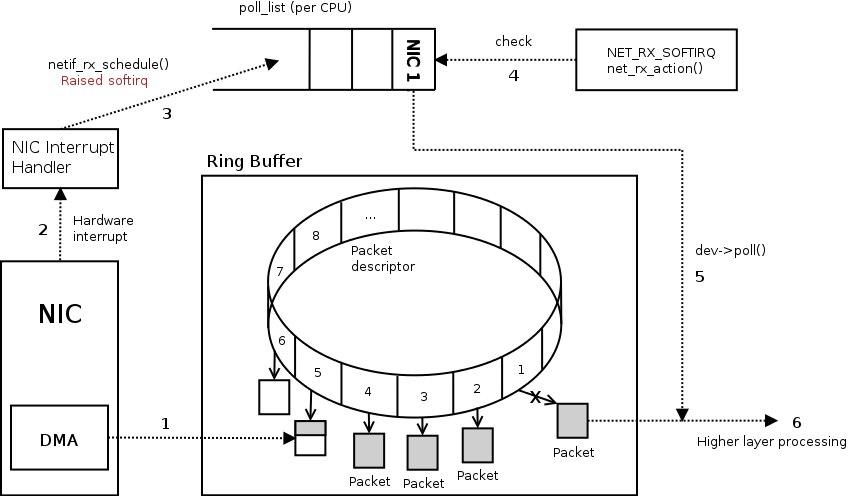
\includegraphics[width=15cm,keepaspectratio]{fig/napi-workflow.png}
	\caption{NAPI workflow}
	\label{fig:linux-napi-workflow}
\end{figure}

When the kernel is ready to deal with more packets, the {\it{poll()}} function of the next device
in the {\it{poll\_list}} will be called.
The scheduled devices are probed in a round-robin manner.
The total number of packets fetched from devices in the {\it{poll\_list}} is limited.
If it was not sufficient to serve all devices in the {\it{poll\_list}} and the kernel should release the CPU,
the devices have to wait for the next NET\_RX\_SOFTIRQ run~\cite{understanding-internals}.
The softirq NET\_RX\_SOFTIRQ processing for NAPI-compliant drivers
is implement by the {\it{net\_rx\_action()}} function defined in {\it{net/core/dev.c}}~\cite{kernel-source}.
The function overview is shown in figure~\ref{fig:linux-softirq-napi}.

\begin{figure}
	\centering
	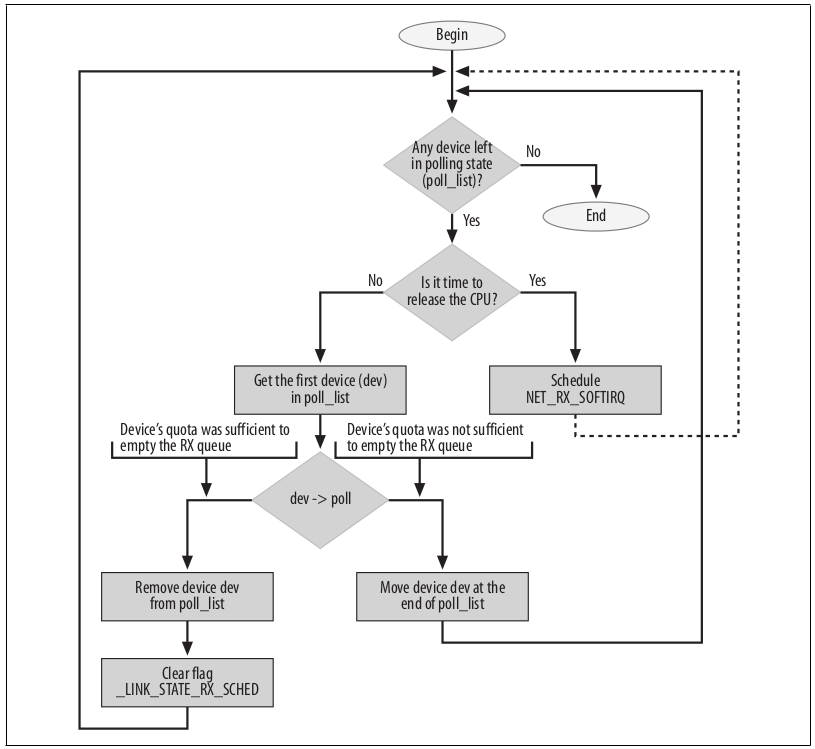
\includegraphics[width=14.5cm,keepaspectratio]{fig/net_rq_softirq.png}
	\caption{Softirq NAPI routine {\it{net\_rx\_action}} (source:~\cite{understanding-internals})}
	\label{fig:linux-softirq-napi}
\end{figure}

When a device driver uses NAPI, it is up to
the driver to implement any congestion control mechanism.
This is because ingress frames are kept in the NIC's memory or in the receive ring buffer managed by the driver,
and the kernel cannot keep track of traffic congestion~\cite{understanding-internals}.
When the host becomes congested, the packets are lost because of not enough space in the ring buffer.
The packets that are going to be lost are not fed into the network stack, so they take no CPU time~\cite{haifux-lecture}.

When a device cannot clear out its ingress queue in a single poll,
it has to wait until the next call.
The kernel keeps calling the driver's {\it{poll()}} function until
it empties the device's ingress queue out~\cite{understanding-internals}.
At that point, there is no need anymore for polling.
The device is removed from the {\it{poll\_list}}
and the device driver can re-enable interrupt notifications for the device~\cite{understanding-internals}.
Nowadays, almost every driver supports the NAPI feature~\cite{linux-kernel-networking}.

NAPI reduces interrupt load on the system and lowers the CPU utilisation under heavy load,
but it increases latency as packets are not processed as quickly~\cite{linux-foundation-napi}.
User-space applications that need the lowest
possible latency and are willing to pay a cost of higher CPU utilisation,
can use a capability for busy polling on sockets (called Low Latency Sockets), which was added in kernel 3.11~\cite{linux-kernel-networking}.
Low Latency Sockets eliminate the cost of the interrupt and context switch
and provide latency very close to the hardware latency~\cite{intel-lls}.

In addition to NAPI, various offload engines were designed to take over some responsibilities of the networking code
and implement them in hardware.
